% Options for packages loaded elsewhere
\PassOptionsToPackage{unicode}{hyperref}
\PassOptionsToPackage{hyphens}{url}
%
\documentclass[
  letterpaper,
  ignorenonframetext,
  aspectratio=43,
  handout,
  12pt]{beamer}
\usepackage{pgfpages}
\setbeamertemplate{caption}[numbered]
\setbeamertemplate{caption label separator}{: }
\setbeamercolor{caption name}{fg=normal text.fg}
\beamertemplatenavigationsymbolsempty
% Prevent slide breaks in the middle of a paragraph
\widowpenalties 1 10000
\raggedbottom
\setbeamertemplate{part page}{
  \centering
  \begin{beamercolorbox}[sep=16pt,center]{part title}
    \usebeamerfont{part title}\insertpart\par
  \end{beamercolorbox}
}
\setbeamertemplate{section page}{
  \centering
  \begin{beamercolorbox}[sep=12pt,center]{part title}
    \usebeamerfont{section title}\insertsection\par
  \end{beamercolorbox}
}
\setbeamertemplate{subsection page}{
  \centering
  \begin{beamercolorbox}[sep=8pt,center]{part title}
    \usebeamerfont{subsection title}\insertsubsection\par
  \end{beamercolorbox}
}
\AtBeginPart{
  \frame{\partpage}
}
\AtBeginSection{
  \ifbibliography
  \else
    \frame{\sectionpage}
  \fi
}
\AtBeginSubsection{
  \frame{\subsectionpage}
}
\usepackage{amsmath,amssymb}
\usepackage{lmodern}
\usepackage{ifxetex,ifluatex}
\ifnum 0\ifxetex 1\fi\ifluatex 1\fi=0 % if pdftex
  \usepackage[T1]{fontenc}
  \usepackage[utf8]{inputenc}
  \usepackage{textcomp} % provide euro and other symbols
\else % if luatex or xetex
  \usepackage{unicode-math}
  \defaultfontfeatures{Scale=MatchLowercase}
  \defaultfontfeatures[\rmfamily]{Ligatures=TeX,Scale=1}
\fi
\usetheme[]{metropolis}
% Use upquote if available, for straight quotes in verbatim environments
\IfFileExists{upquote.sty}{\usepackage{upquote}}{}
\IfFileExists{microtype.sty}{% use microtype if available
  \usepackage[]{microtype}
  \UseMicrotypeSet[protrusion]{basicmath} % disable protrusion for tt fonts
}{}
\makeatletter
\@ifundefined{KOMAClassName}{% if non-KOMA class
  \IfFileExists{parskip.sty}{%
    \usepackage{parskip}
  }{% else
    \setlength{\parindent}{0pt}
    \setlength{\parskip}{6pt plus 2pt minus 1pt}}
}{% if KOMA class
  \KOMAoptions{parskip=half}}
\makeatother
\usepackage{xcolor}
\IfFileExists{xurl.sty}{\usepackage{xurl}}{} % add URL line breaks if available
\IfFileExists{bookmark.sty}{\usepackage{bookmark}}{\usepackage{hyperref}}
\hypersetup{
  hidelinks,
  pdfcreator={LaTeX via pandoc}}
\urlstyle{same} % disable monospaced font for URLs
\newif\ifbibliography
\usepackage{graphicx}
\makeatletter
\def\maxwidth{\ifdim\Gin@nat@width>\linewidth\linewidth\else\Gin@nat@width\fi}
\def\maxheight{\ifdim\Gin@nat@height>\textheight\textheight\else\Gin@nat@height\fi}
\makeatother
% Scale images if necessary, so that they will not overflow the page
% margins by default, and it is still possible to overwrite the defaults
% using explicit options in \includegraphics[width, height, ...]{}
\setkeys{Gin}{width=\maxwidth,height=\maxheight,keepaspectratio}
% Set default figure placement to htbp
\makeatletter
\def\fps@figure{htbp}
\makeatother
% Make links footnotes instead of hotlinks:
\DeclareRobustCommand{\href}[2]{#2\footnote{\url{#1}}}
\setlength{\emergencystretch}{3em} % prevent overfull lines
\providecommand{\tightlist}{%
  \setlength{\itemsep}{0pt}\setlength{\parskip}{0pt}}
\setcounter{secnumdepth}{-\maxdimen} % remove section numbering
\usepackage{pgfpages}
\pgfpagesuselayout{2 on 1}
\providecommand{\tightlist}{%
\setlength{\itemsep}{0pt}\setlength{\parskip}{0pt}}
\makeatletter
\makeatother
\let\Oldincludegraphics\includegraphics
\renewcommand{\includegraphics}[2][]{\Oldincludegraphics[width=\textwidth,height=0.7\textheight,keepaspectratio]{#2}}
\ifluatex
  \usepackage{selnolig}  % disable illegal ligatures
\fi

\author{}
\date{}

\begin{document}

\begin{frame}{AE 737: Mechanics of Damage Tolerance}
\protect\hypertarget{ae-737-mechanics-of-damage-tolerance}{}
Lecture 5 - Plastic Zone

Dr.~Nicholas Smith

Wichita State University, Department of Aerospace Engineering

February 15, 2021
\end{frame}

\begin{frame}{schedule}
\protect\hypertarget{schedule}{}
\begin{itemize}
\tightlist
\item
  15 Feb - Plastic Zone
\item
  17 Feb - Plastic Zone, HW 2 Due, HW 1 Self-grade due
\item
  22 Feb - Fracture Toughness
\item
  24 Feb - Fracture Toughness, HW3 Due, HW 2 Self-grade due
\end{itemize}
\end{frame}

\begin{frame}{outline}
\protect\hypertarget{outline}{}
\begin{itemize}
\tightlist
\item
  curved boundaries
\item
  stress concentration factors
\item
  plastic zone
\end{itemize}
\end{frame}

\hypertarget{curved-boundaries}{%
\section{curved boundaries}\label{curved-boundaries}}

\begin{frame}{short cracks on curved boundaries}
\protect\hypertarget{short-cracks-on-curved-boundaries}{}
\begin{itemize}
\tightlist
\item
  For short cracks, we can use the \emph{stress concentration factor} on
  a curved boundary to determine the stress intensity factor
\item
  The stress concentration factor only gives the maximum stress at the
  curved boundary, thus the longer the crack is, the farther away from
  the curved boundary (and maximum stress) it is.
\item
  Stress concentration factors can be found: pp.~82-85 in the text
\item
  Also see supplemental text on Blackboard or
  \href{../classdocs/stress_concentrations.pdf}{here}
\end{itemize}
\end{frame}

\begin{frame}{short cracks on curved boundaries}
\protect\hypertarget{short-cracks-on-curved-boundaries-1}{}
\begin{itemize}
\tightlist
\item
  Suppose we want to determine the stress intensity on a panel, panel B
\item
  We find a similar panel with a known stress intensity factor, panel A
\item
  We adjust the applied load on panel A such that
  \emph{K}\emph{I},\emph{A}=\emph{K}\emph{I},\emph{B}
\item
  The magnitude of this load adjustment is determined using the
  \emph{stress concentration factors} in panels B and A Note: the
  notation: K\_t for stress concentration factor, K\_I for stress
  intensity factor
\end{itemize}
\end{frame}

\begin{frame}{short cracks on curved boundaries}
\protect\hypertarget{short-cracks-on-curved-boundaries-2}{}
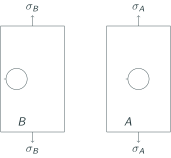
\includegraphics{../images/curved-short.svg}
\end{frame}

\begin{frame}{short cracks on curved boundaries}
\protect\hypertarget{short-cracks-on-curved-boundaries-3}{}
\begin{itemize}
\tightlist
\item
  Since \emph{A} is a fictional panel, we set the applied stress,
  \(\sigma_A\) such that
\end{itemize}

\[\sigma_{max,B} = \sigma_{max,A}\]

\begin{itemize}
\tightlist
\item
  Substituting stress concentration factors
\end{itemize}

\[K_{t,B} \sigma_B = K_{t,A} \sigma_A\]

\begin{itemize}
\tightlist
\item
  Solving for \(\sigma_A\)
\end{itemize}

\[\sigma_A = \frac{K_{t,B}}{K_{t,A}}\sigma_B\]
\end{frame}

\begin{frame}{short cracks on curved boundaries}
\protect\hypertarget{short-cracks-on-curved-boundaries-4}{}
\begin{itemize}
\tightlist
\item
  Since the crack is short and \(\sigma_{max, A} = \sigma_{max, B}\) we
  can say
\end{itemize}

\[\begin{aligned}
  K_{I,B} &= K_{I,A}\\
  &= \sigma_A \sqrt{\pi c} \beta_A\\
  &= \frac{K_{t,B}}{K_{t,A}}\sigma_B \sqrt{\pi c} \beta_A
\end{aligned}\]
\end{frame}

\begin{frame}{example 6 (p.~86)}
\protect\hypertarget{example-6-p.-86}{}
\begin{figure}
\centering
\includegraphics{../images/example-86-6.jpg}
\caption{See p.~86, there is a short through crack on the edge of a 0.5"
deep notch on a 5 inch wide panel with a remote 12 ksi stress applied.
The net section stress concentration factor is 2.8, while the global
stress concentration factor for a similar panel with a hole is 3.1}
\end{figure}
\end{frame}

\begin{frame}{long cracks on curved boundaries}
\protect\hypertarget{long-cracks-on-curved-boundaries}{}
\begin{itemize}
\tightlist
\item
  As a crack becomes very large, the effect of the curved boundary
  diminishes
\item
  We find expressions for \(\beta_L\) (long crack) and \(\beta_S\)
  (short crack)
\item
  We connect \(\beta_S\) to \(\beta_L\) using a straight line from
  \(\beta_S\) to a tangent intersection with \(\beta_L\)
\end{itemize}
\end{frame}

\begin{frame}{long cracks on curved boundaries}
\protect\hypertarget{long-cracks-on-curved-boundaries-1}{}
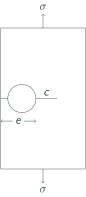
\includegraphics{../images/curved-long.svg}
\end{frame}

\begin{frame}{example}
\protect\hypertarget{example}{}
\begin{itemize}
\tightlist
\item
  Example
  \href{../examples/Long\%20Cracks\%20on\%20Curved\%20Boundaries.html}{here}
\end{itemize}
\end{frame}

\begin{frame}{group one}
\protect\hypertarget{group-one}{}
\begin{columns}[T]
\begin{column}{0.5\textwidth}
\includegraphics{../images/curved-group1.svg}
\end{column}

\begin{column}{0.5\textwidth}
\begin{itemize}
\tightlist
\item
  \emph{c} = 0.75, \emph{e} = 2.25, \emph{r} = 0.5
\item
  assume \emph{a} is short and calculate \(\beta\) for this case
\item
  calculate in terms of \(\beta\) for known state
\end{itemize}
\end{column}
\end{columns}
\end{frame}

\begin{frame}{group two}
\protect\hypertarget{group-two}{}
\begin{columns}[T]
\begin{column}{0.5\textwidth}
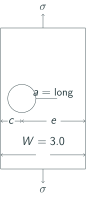
\includegraphics{../images/curved-group2.svg}
\end{column}

\begin{column}{0.5\textwidth}
\begin{itemize}
\tightlist
\item
  \emph{c} = 0.75, \emph{e} = 2.25, \emph{r} = 0.5
\item
  assume \emph{a} is long and calculate \(\beta\) for this case
\item
  calculate in terms of \(\beta\) for known state
\end{itemize}
\end{column}
\end{columns}
\end{frame}

\begin{frame}{group three}
\protect\hypertarget{group-three}{}
\begin{columns}[T]
\begin{column}{0.5\textwidth}
\includegraphics{../images/curved-group3.svg}
\end{column}

\begin{column}{0.5\textwidth}
\begin{itemize}
\tightlist
\item
  \emph{c} = 0.75, \emph{e} = 2.25, \emph{r} = 0.5
\item
  assume \emph{a} is short and calculate \(\beta\) for this case
\item
  calculate in terms of \(\beta\) for known state
\end{itemize}
\end{column}
\end{columns}
\end{frame}

\begin{frame}{group four}
\protect\hypertarget{group-four}{}
\begin{columns}[T]
\begin{column}{0.5\textwidth}
\includegraphics{../images/curved-group4.svg}
\end{column}

\begin{column}{0.5\textwidth}
\begin{itemize}
\tightlist
\item
  \emph{c} = 0.75, \emph{e} = 2.25, \emph{r} = 0.5
\item
  assume \emph{a} is long and calculate \(\beta\) for this case
\item
  calculate in terms of \(\beta\) for known state
\end{itemize}
\end{column}
\end{columns}
\end{frame}

\begin{frame}{discussion}
\protect\hypertarget{discussion}{}
Draw a sketch to show how we could use this method to find cracks of
intermediate length near a curved boundary
\end{frame}

\hypertarget{stress-concentration-factors}{%
\section{stress concentration
factors}\label{stress-concentration-factors}}

\begin{frame}{centered hole tension - p.~82}
\protect\hypertarget{centered-hole-tension---p.-82}{}
\begin{figure}
\centering
\includegraphics{../images/kt-hole.png}
\caption{A plot of stress concentration factors near a hole, see text
p.~82 or the interactive plots linked in the last slide.}
\end{figure}

\(K_{tg}\) uses stress for the cross-sectional area if no hole was
present, \(K_{tn}\) uses stress at the net section (subtracting hole
area). \emph{a} is the hole diameter, \emph{W} is specimen width.
\end{frame}

\begin{frame}{off-center hole tension - p.~83}
\protect\hypertarget{off-center-hole-tension---p.-83}{}
\includegraphics{../images/Kt-offcenter-hole.png}

\(K_{tg}\) uses stress for the cross-sectional area if no hole was
present, \(K_{tn}\) uses stress at the net section (subtracting hole
area). c is the distance from the closest edge to the center of the
hole, e is the distance from the farthest edge to the center of the
hole, r is hole radius.
\end{frame}

\begin{frame}{bending of a bar with u-shaped notch - p.~84}
\protect\hypertarget{bending-of-a-bar-with-u-shaped-notch---p.-84}{}
\begin{figure}
\centering
\includegraphics{../images/kt-bending-edge.png}
\caption{A plot of stress concentration factors in a bar with a u-shaped
notch, see text p.~84 or the interactive plots linked in the last
slide.}
\end{figure}

Nominal stress used for \(K_t\) is given by \(\sigma_{nom} = 6M/hd^2\)
where \emph{M} is applied bending moment, \emph{h} is thickness,
\emph{d} is the net-section height (height minus notch depth). \emph{D}
is the height of the panel without a notch and \emph{r} is the notch
radius.
\end{frame}

\begin{frame}{tension of a stepped bar with shoulder fillets - p.~85}
\protect\hypertarget{tension-of-a-stepped-bar-with-shoulder-fillets---p.-85}{}
\includegraphics{../images/fillet.png}

\emph{D} is the larger width (before the step), \emph{d} is the width
after the step. Nominal stress is \(\sigma_{nom} = P/hd\), where
\emph{h} is specimen thickness. \emph{r} is the fillet radius.
\end{frame}

\begin{frame}{interactive page}
\protect\hypertarget{interactive-page}{}
\begin{itemize}
\tightlist
\item
  An interactive page with these plots can be accessed
  \href{../examples/Stress\%20Concentration\%20Factors.html}{here}
\end{itemize}
\end{frame}

\hypertarget{plastic-zone}{%
\section{plastic zone}\label{plastic-zone}}

\begin{frame}{plastic zone}
\protect\hypertarget{plastic-zone-1}{}
\begin{itemize}
\tightlist
\item
  Previous developments assumed perfectly elastic materials
\item
  Most common materials have some plasticity
\item
  Any stress above the yield stress will undergo plastic deformation (no
  stress higher than \(\sigma_y\) will be present in the material)
\end{itemize}
\end{frame}

\begin{frame}{plastic zone}
\protect\hypertarget{plastic-zone-2}{}
\begin{itemize}
\tightlist
\item
  Plasticity helps retard crack propagation due to residual stresses
\item
  After an overload, elastic regions will contract back to their
  undeformed shape
\item
  The region which has undergone plastic deformation, however, holds its
  deformed shape
\item
  This introduces a region of residual compressive stress near the crack
  tip
\item
  Before the crack can propagate, a stress needs to overcome this
  residual stress
\end{itemize}
\end{frame}

\begin{frame}{2D problems}
\protect\hypertarget{d-problems}{}
\begin{itemize}
\tightlist
\item
  We often simplify the full 3D elasticity equations for planar problems
\item
  For very thin panels, we assume that all out-of-plane stresses are 0
\item
  This is called plane stress
\end{itemize}
\end{frame}

\begin{frame}{plane stress}
\protect\hypertarget{plane-stress}{}
\[\begin{aligned}
  \sigma_z &= \tau_{xz} = \tau_{zy} = 0\\
  \epsilon_x &= \frac{\sigma_x}{E} - \nu \frac{\sigma_y}{E}\\
  \epsilon_y &= -\nu \frac{\sigma_x}{E} + \frac{\sigma_y}{E}\\
  \epsilon_z &= -\nu \frac{\sigma_x}{E} - \nu \frac{\sigma_y}{E}\\
  \gamma_{xy} &= \frac{\tau_{xy}}{G}\\
  \gamma_{xz} &= \gamma_{yz} = 0
\end{aligned}\]
\end{frame}

\begin{frame}{2D problems}
\protect\hypertarget{d-problems-1}{}
\begin{itemize}
\tightlist
\item
  When instead a panel is very thick, we assume that any strains through
  the thickness are small relative to other strains
\item
  \(\epsilon_z = \gamma_{xz} = \gamma_{yz} = 0\)
\item
  This is known as plane strain
\end{itemize}
\end{frame}

\begin{frame}{plane strain}
\protect\hypertarget{plane-strain}{}
\[\begin{aligned}
  \epsilon_x &= \frac{\sigma_x}{E} - \nu \frac{\sigma_y}{E} - \nu \frac{\sigma_z}{E}\\
  \epsilon_y &= -\nu \frac{\sigma_x}{E} + \frac{\sigma_y}{E} - \nu \frac{\sigma_z}{E}\\
  0 &= -\nu \frac{\sigma_x}{E} - \nu \frac{\sigma_y}{E} + \frac{\sigma_z}{E}\\
  \gamma_{xy} &= \frac{\tau_{xy}}{G}\\
  \gamma_{xz} &= \gamma_{yz} = 0
\end{aligned}\]
\end{frame}

\begin{frame}{Irwin's first approximation}
\protect\hypertarget{irwins-first-approximation}{}
\begin{itemize}
\tightlist
\item
  If we recall the equation for opening stress (\(\sigma_y\)) near the
  crack tip
\end{itemize}

\[\sigma_y = \frac{K_I}{\sqrt{2\pi r}} \cos \frac{\theta}{2} \left(1+\sin \frac{\theta}{2}\sin \frac{3\theta}{2}\right) \tag{1.2}\]

\begin{itemize}
\tightlist
\item
  In the plane of the crack, when \(\theta=0\) we find
\end{itemize}

\[\sigma_y = \frac{K_I}{\sqrt{2\pi r}}\]
\end{frame}

\begin{frame}{Irwin's first approximation}
\protect\hypertarget{irwins-first-approximation-1}{}
\includegraphics{../images/plastic-zone.svg}
\end{frame}

\begin{frame}{Irwin's first approximation}
\protect\hypertarget{irwins-first-approximation-2}{}
\begin{columns}[T]
\begin{column}{0.5\textwidth}
\begin{itemize}
\tightlist
\item
  We use \emph{C}, the \emph{Plastic Constraint Factor} to convert
  between Plane Strain and Plane Stress solutions
\item
  The plastic zone size can now be approximated
\end{itemize}
\end{column}

\begin{column}{0.5\textwidth}
\[\begin{aligned}
  \sigma_{yy}(r=r_p) &= C\sigma_{YS}\\
  \frac{K_I}{\sqrt{2\pi r_p}} &= C\sigma_{YS}\\
  r_p &= \frac{1}{2\pi} \left(\frac{K_I}{C\sigma_{YS}}\right)^2
\end{aligned}\]
\end{column}
\end{columns}
\end{frame}

\begin{frame}{Irwin's first approximation}
\protect\hypertarget{irwins-first-approximation-3}{}
\begin{itemize}
\tightlist
\item
  For plane stress (thin panels) we let \(C=1\) and find
  \emph{r}\emph{p} as
\end{itemize}

\[r_p = \frac{1}{2\pi} \left(\frac{K_I}{\sigma_{YS}}\right)^2\]

\begin{itemize}
\tightlist
\item
  And for plane strain (thick panels) we let \(C=\sqrt{3}\) and find
\end{itemize}

\[r_p = \frac{1}{6\pi} \left(\frac{K_I}{\sigma_{YS}}\right)^2\]
\end{frame}

\begin{frame}{Intermediate panels}
\protect\hypertarget{intermediate-panels}{}
\begin{itemize}
\tightlist
\item
  For panels which lie between plane strain and plane stress states, we
  use the following expression to estimate the plastic zone size
\end{itemize}

\[r_p = \frac{1}{I\pi} \left(\frac{K_I}{\sigma_{YS}}\right)^2\]

\begin{itemize}
\tightlist
\item
  Where \emph{I} is defined as
\end{itemize}

\[I = 6.7 - \frac{1.5}{t}\left(\frac{K_I}{\sigma_{YS}}\right)^2\]

\begin{itemize}
\tightlist
\item
  And \(2 \le I \le 6\)
\end{itemize}
\end{frame}

\begin{frame}{Irwin's second approximation}
\protect\hypertarget{irwins-second-approximation}{}
\begin{itemize}
\tightlist
\item
  If our material is perfectly elastic-plastic, no stresses above
  \(C\sigma_{ys}\) will exist in the material
\item
  This ignores the strain energy (represented by the area under the
  curve) in the plastic zone
\end{itemize}
\end{frame}

\begin{frame}{Irwin's second approximation}
\protect\hypertarget{irwins-second-approximation-1}{}
\includegraphics{../images/plastic-missing.svg}
\end{frame}

\begin{frame}{Irwin's second approximation}
\protect\hypertarget{irwins-second-approximation-2}{}
\begin{itemize}
\tightlist
\item
  To account for the additional strain energy, Irwin considered a
  plastic zone size increased by some \(\delta\)
\item
  He also needed to adjust the stress function, and considered an
  equivalent crack tip in these calculations
\end{itemize}
\end{frame}

\begin{frame}{Irwin's second approximation}
\protect\hypertarget{irwins-second-approximation-3}{}
\includegraphics{../images/plastic-equivalent.svg}
\end{frame}

\begin{frame}{Irwin's second approximation}
\protect\hypertarget{irwins-second-approximation-4}{}
\begin{columns}[T]
\begin{column}{0.5\textwidth}
We need \emph{A}=\emph{B}, so we set them equivalent and solve for
\(\delta\).
\end{column}

\begin{column}{0.5\textwidth}
\[\begin{aligned}
  A &= \int_{0}^{r_p} \sigma_{yy} dr - r_p \sigma_{YS}\\
  &= \int_{0}^{r_p} \frac{K_I}{\sqrt{2\pi r}} dr - r_p \sigma_{YS}\\
  &= \frac{K_I}{\sqrt{2\pi}}\int_{0}^{r_p} r^{-1/2} dr - r_p \sigma_{YS}\\
  &= \frac{2K_I \sqrt{r_p}}{\sqrt{2\pi}}- r_p \sigma_{YS}
\end{aligned}\]
\end{column}
\end{columns}
\end{frame}

\begin{frame}{Irwin's second approximation}
\protect\hypertarget{irwins-second-approximation-5}{}
\begin{itemize}
\tightlist
\item
  We have already found \emph{r}\emph{p} as
\end{itemize}

\[r_p = \frac{1}{2\pi} \left(\frac{K_I}{\sigma_{YS}}\right)^2\]

\begin{itemize}
\tightlist
\item
  If we solve this for \emph{K}\emph{I} we find
\end{itemize}

\[K_I = \sqrt{2\pi r_p} \sigma_{YS}\]
\end{frame}

\begin{frame}{Irwin's second approximation}
\protect\hypertarget{irwins-second-approximation-6}{}
\begin{itemize}
\tightlist
\item
  We can now substitute back into the strain energy of A
\end{itemize}

\[\begin{aligned}
  A &= \frac{2\sqrt{2\pi r_p} \sigma_{YS} \sqrt{r_p}}{\sqrt{2\pi}}- r_p \sigma_{YS}\\
  &= 2 \sigma_{YS} r_p- r_p \sigma_{YS}\\
  &= r_p \sigma_{YS}
\end{aligned}\]
\end{frame}

\begin{frame}{Irwin's second approximation}
\protect\hypertarget{irwins-second-approximation-7}{}
\begin{itemize}
\tightlist
\item
  B is given simply as \(B=\delta \sigma_{ys}\) so we equate A and B to
  find \$\delta\$
\end{itemize}

\[\begin{aligned}
  A &= B\\
  r_p \sigma_{YS} &= \delta \sigma_{YS}\\
  r_p &= \delta
\end{aligned}\]
\end{frame}

\begin{frame}{Irwin's second approximation}
\protect\hypertarget{irwins-second-approximation-8}{}
\begin{itemize}
\tightlist
\item
  This means the plastic zone size is simply 2\emph{r}\emph{p}
\item
  However, it also means that the effective crack length is
  \emph{a}+\emph{r}\emph{p}
\item
  Since \emph{r}\emph{p} depends on \emph{K}\emph{I}, we must iterate a
  bit to find the ``real'' \emph{r}\emph{p} and \emph{K}\emph{I}
\end{itemize}
\end{frame}

\begin{frame}{Example}
\protect\hypertarget{example-1}{}
\begin{figure}
\centering
\includegraphics{../images/plastic-example.svg}
\caption{An edge crack of length a in a panel of width W is subjected to
a remote load}
\end{figure}
\end{frame}

\begin{frame}{equations}
\protect\hypertarget{equations}{}
\[\begin{aligned}
  \beta &= \left[1.122 - 0.231 \frac{a}{W} + 10.55 \left(\frac{a}{W}\right)^2 - 21.71 \left(\frac{a}{W}\right)^3 + 30.82 \left(\frac{a}{W}\right)^4\right] \\
  I &= 6.7 - \frac{1.5}{t}\left(\frac{K_I}{\sigma_{YS}}\right)^2 \\
  r_p &= \frac{1}{I\pi} \left(\frac{K_I}{\sigma_{YS}}\right)^2
\end{aligned}\]
\end{frame}

\end{document}
